\documentclass[11pt]{article}
\usepackage[margin=1in]{geometry}
\usepackage{graphicx}
\usepackage{booktabs}
\usepackage{tabularx}
\usepackage{amsmath,amssymb}
\usepackage[font=small,labelfont=bf]{caption}
\usepackage{xcolor}
\usepackage{enumitem}
\usepackage{float}
\usepackage[section]{placeins}
\usepackage[colorlinks=true,linkcolor=blue!50!black,citecolor=blue!50!black,urlcolor=blue!50!black]{hyperref}
\setlist{itemsep=1pt,topsep=3pt}
\emergencystretch=2em
\newcolumntype{Y}{>{\raggedright\arraybackslash}X}
\newcommand{\obs}{\textnormal{\textsc{[obs]}}}
\newcommand{\pred}{\textnormal{\textsc{[pred]}}}
\newcommand{\ext}{\textnormal{\textsc{[ext]}}}
\newcommand{\code}[1]{\texttt{\small #1}}
\newcommand{\studentbox}[1]{\par\smallskip\noindent\fcolorbox{orange!70!black}{orange!8}{\parbox{\dimexpr\linewidth-2\fboxsep-2\fboxrule}{\small\textbf{Student verification (to complete before submission):} #1}}\par\smallskip}

\title{Structural, Single-Cell and Spatial Analyses with an AI Agent Workspace:\\
EGFR Variants, PBMC3k Robustness and Mouse-Brain Spatial Domains}
\author{[Student Name] \\ \small CMU 11-781 / 02-741 Generative AI for Biomedicine, Assignment 3, Fall 2026}
\date{October 2026}

\begin{document}
\maketitle

\begin{abstract}
We used an AI agent workspace (Claude Code, model Claude Opus 5.5) to carry out three analyses and audited its work.
\textbf{(1)} For EGFR variants G719S, T790M and L858R we mapped canonical positions onto PDB 4HJO (whose numbering is canonical $-24$) and measured their structural context. L858R has the most direct structural support for a mechanism (burial in the inactive state), T790M sits at the drug pocket but a drug-bound Met790 structure shows no steric clash, and G719S evidence is indirect.
\textbf{(2)} PBMC3k clustering gives nine populations. B cells are robust to resolution and subsampling; the CD8\,T/NK split depends on resolution; the naive/memory CD4 boundary is a continuum, and the ``naive CD4'' cluster contains an estimated 31--40\% CD8 T cells.
\textbf{(3)} Expression-only Visium domains are strongly spatially coherent (same-domain edge fraction 0.783 vs 0.084 under 1{,}000 label permutations, $p=0.001$), and this survives depth/mitochondrial regression (ARI 0.78). Moran's I and Wilcoxon DE rankings agree only moderately ($\rho=0.52$), and less when DE is ranked by fold change ($\rho=0.29$).
All results are regenerated by one script in about four minutes on a CPU.
\end{abstract}

\section{Introduction}
The assignment asks whether an agent workspace can produce biomedical analyses that are correct, checkable and honestly qualified. We address three tasks: a protein-structure interpretation of three clinically important EGFR mutations, a robustness study of single-cell clustering, and a test of whether expression-defined spatial domains are organised in tissue. Throughout, claims are tagged as observations computed here \obs, predictions or interpretations \pred, or retrieved external evidence \ext. The agent's own errors, and the checks that caught them, are reported in Appendix~\ref{app:audit}.

\section{Methods}
\paragraph{Workspace and reproducibility.} The agent wrote and ran all code (\code{submission/*/code/}) on a CPU-only Linux machine; no GPU or structure prediction was run. \code{run\_all.sh} creates a Python 3.12 environment with \code{uv} from \code{requirements.txt}, downloads and SHA-256-checks every input (\code{fetch\_data.sh}), runs the 11 analysis scripts in order and compiles this report. Key software: scanpy 1.12.5, squidpy 1.8.4, leidenalg 0.12.0, scikit-learn 1.9.1, gemmi 0.7.5, Biopython 1.88, freesasa 2.2.1, PyMOL 3.2.

\paragraph{Protein (Task 1).} UniProt P00533 (entry v301) supplied the canonical sequence and annotations. Each structure's full SEQRES was aligned globally to UniProt (BLOSUM62) to map residues; the depositors' SEQADV records were used as a cross-check. Structures: 4HJO (primary; WT+V948R, erlotinib, inactive, 2.75\,\AA~\cite{park2012}), 1M17 (WT, erlotinib, active-like~\cite{stamos2002}), 2ITX/2ITN/2ITV (WT/G719S/L858R with AMP-PNP~\cite{yun2007}), 2JIT (T790M apo~\cite{yun2008}), 4I22 (L858R/T790M/V948R, gefitinib~\cite{gajiwala2013}) and the AlphaFold DB model~\cite{jumper2021}. Measurements use heavy atoms only: minimum inter-atomic distance, residues within 5\,\AA, relative SASA (freesasa, 1.4\,\AA\ probe, ligands removed) and $\alpha$C state from the K745\,NZ--E762\,OE distance ($<4$\,\AA\ = $\alpha$C-in).

\paragraph{Single cell (Task 2).} PBMC3k (10x Genomics~\cite{zheng2017}). QC: 200--2{,}500 genes, $<5\%$ mitochondrial reads, genes in $\ge 3$ cells. Then normalisation to $10^4$, log1p, 2{,}000 HVGs (Seurat flavour), regression of total counts and \% mito, scaling, PCA (30 PCs), kNN ($k=15$), Leiden~\cite{traag2019} and UMAP, all with seed 0~\cite{wolf2018}. Labels come from Wilcoxon markers computed on these data plus a rule that scores literature marker sets per cluster and reports a cluster as ambiguous if the top two scores differ by $<0.15$; no reference labels were used. Robustness: Leiden at resolutions 0.3, 0.6, 1.0, 1.4 on the same graph; a 70\% cell subsample (seed 42) re-run from raw counts; extra Leiden seeds and subsample seeds 1--5.

\paragraph{Spatial (Task 3).} Visium V1 adult mouse brain (10x Genomics). QC: $\ge 5{,}000$ UMIs, $\ge 1{,}000$ genes, $<30\%$ mito. Domains were found by clustering an AnnData object built from counts only (assertions check that no coordinates or image are present): seurat\_v3 HVGs, PCA (30), kNN ($k=15$), Leiden (resolution 0.5, seed 0). The physical-neighbour graph is the Visium hexagonal lattice (squidpy~\cite{palla2022} \code{spatial\_neighbors}, grid, 6 neighbours, first ring). The main statistic is the fraction of graph edges joining two spots of the same domain. The null permutes domain labels across spots on the fixed graph (1{,}000 times, seed 0; one-sided empirical $p=(1+\#\{\text{null}\ge\text{obs}\})/(N+1)$). Spatially variable genes: Moran's I on the 200 top HVGs; DE: Wilcoxon one-vs-rest across domains on the same genes.

\section{Results}

\subsection{EGFR: G719S, T790M and L858R}
\paragraph{Mapping \obs.}\phantomsection\label{sec:map} All three wild-type residues match UniProt. 4HJO and 1M17 use mature-protein numbering (canonical $-24$; L858 is Leu834 in 4HJO), while the 2IT*/2JIT/4I22 entries use canonical numbering. In every structure the only mismatches against UniProt are the deposited mutations, including the engineered V948R of 4HJO, which lies 26--31\,\AA\ from all three sites (Appendix Table~\ref{tab:p1}). AlphaFold confidence is high at T790 (pLDDT 88) but low at L858 (51), consistent with a conformationally variable activation loop.

\paragraph{Structural context \obs.} In inactive 4HJO, \textbf{T790} is the residue closest to erlotinib (3.48\,\AA) and is the closest of the three sites to the ligand in all six ligand complexes. \textbf{L858} is buried (relative SASA 0.10 vs 0.15--0.40 in $\alpha$C-in structures), 2.96\,\AA\ from DFG-D855 and 4.57\,\AA\ from $\alpha$C residue M766, in a mostly hydrophobic shell that also contains K745, D855 and K860. \textbf{G719} is the first Gly of the P-loop, solvent-exposed (SASA 0.35) and 5.06\,\AA\ from erlotinib. Variant-specific checks: superposing apo Met790 (2JIT) onto 4HJO suggests a clash with erlotinib (0.6--1.3\,\AA), but drug-bound Met790 in 4I22 sits 3.3--3.5\,\AA\ from the drug, so the clash is a property of the apo rotamer; in the active-like 1M17 pocket the 4I22 side chain comes to 2.5\,\AA. In G719S (2ITN), Ser OG is 5.15\,\AA\ from the nearest phosphate oxygen (no direct hydrogen bond), and the wild-type Gly backbone angles are not glycine-specific. 4I22 is itself $\alpha$C-out yet accommodates Arg858 through salt bridges to D855 and D837, which argues against a simple ``Arg858 is incompatible with the inactive state'' model.

\begin{figure}[t]
\centering
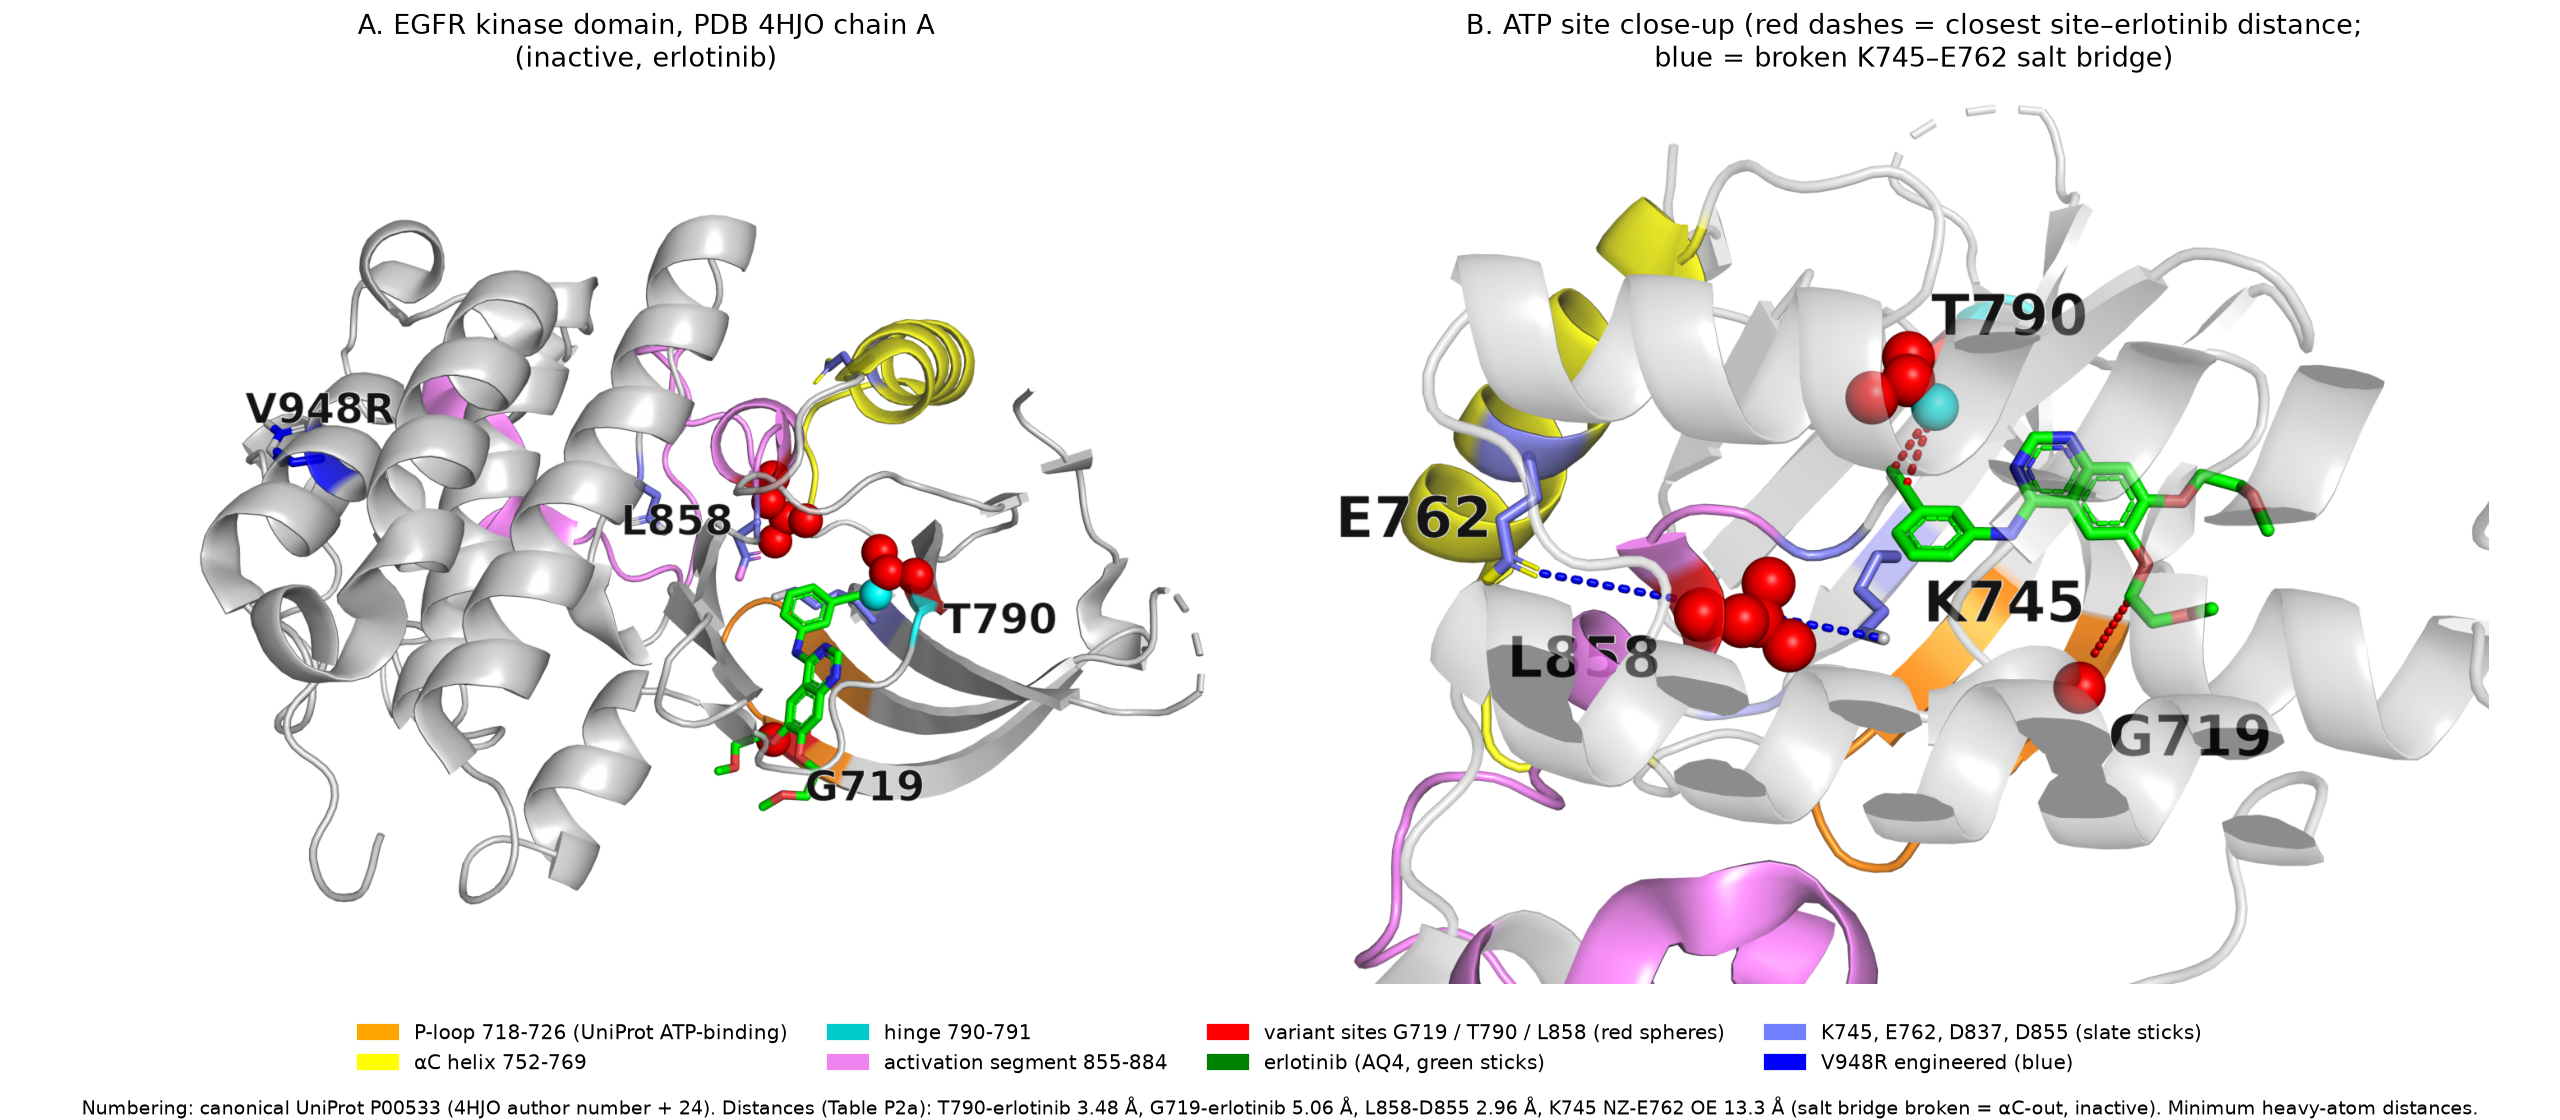
\includegraphics[width=\linewidth]{../protein/outputs/fig_p4_annotated_structure.png}
\caption{\textbf{Annotated EGFR kinase domain (PDB 4HJO, canonical numbering).} (A) Overview; (B) ATP site. Red spheres: variant sites. Green: erlotinib. Red dashes: closest site--erlotinib distances (T790 3.48\,\AA, G719 5.06\,\AA). Blue dashes: broken K745--E762 salt bridge (13.3\,\AA, $\alpha$C-out). Interactive version: \code{egfr\_4hjo\_interactive.html}.}
\label{fig:egfr}
\end{figure}

\begin{table}[t]
\centering\small
\caption{\textbf{Comparison of the three EGFR variants} (measurements from 4HJO unless stated; \code{table\_p2a}, \code{table\_p2d}, \code{table\_p2e}).}
\label{tab:egfr}
\begin{tabularx}{\linewidth}{@{}l Y Y l l@{}}
\toprule
Variant & Structural evidence \obs & Proposed mechanism \pred\ / support \ext & Class & Confidence \\
\midrule
L858R & A-loop helix, buried (SASA 0.10 inactive vs 0.15--0.40 active); 2.96\,\AA\ to D855, 4.57\,\AA\ to $\alpha$C M766; pLDDT 51 & Arg in the pocket that packs the inactive A-loop against $\alpha$C shifts the balance toward the active state~\cite{yun2007,shan2012}. 4I22 shows Arg858 can be accommodated in an $\alpha$C-out state, so it is a shift, not an incompatibility & Activating & Mod.--high \\
\addlinespace
T790M & Gatekeeper; 3.48\,\AA\ to erlotinib; apo Met clashes (0.6--1.3\,\AA) but drug-bound Met does not (3.3--3.5\,\AA) & Resistance mainly via increased ATP affinity~\cite{yun2008,kobayashi2005,pao2005}; our data do not support a purely steric block & Resistance & Moderate \\
\addlinespace
G719S & P-loop Gly (GxGxxG), exposed (SASA 0.35); 5.06\,\AA\ to erlotinib; Ser OG 5.15\,\AA\ to phosphate; P-loop shift $\le$1.95\,\AA & Altered P-loop flexibility destabilises the inactive state~\cite{yun2007}; no new contact or backbone strain observed & Activating & Low--mod. \\
\bottomrule
\end{tabularx}
\end{table}

\paragraph{Interpretation.} Table~\ref{tab:egfr} ranks the variants by how directly the structures support a mechanism: \textbf{L858R $>$ T790M $>$ G719S}. Ranking by functional impact on one scale is not meaningful, because L858R and G719S are activating mutations that predict inhibitor sensitivity~\cite{lynch2004,paez2004}, while T790M confers resistance. AlphaMissense~\cite{cheng2023} scores all three as pathogenic ($\ge 0.96$) and cannot separate these classes.

\subsection{PBMC3k: cell types and their robustness}
\paragraph{Baseline \obs.} QC kept 2{,}638 of 2{,}700 cells (13{,}656 genes). At resolution 1.0, Leiden gives nine clusters (Fig.~\ref{fig:sc}A, Table~\ref{tab:sc}). Resolution 1.0 is the lowest tested value that separates CD8\,T from NK cells; it was chosen after seeing results at 0.6, which we disclose as a researcher degree of freedom.

\begin{table}[t]
\centering\small
\caption{\textbf{Baseline clusters and labels} (resolution 1.0; markers are Wilcoxon log$_2$FC from these data, \code{table\_s2b}; marker biology from~\cite{zheng2017,hao2021,villani2017}).}
\label{tab:sc}
\begin{tabularx}{\linewidth}{@{}r r Y l@{}}
\toprule
Cluster & Cells & Top data-derived markers & Label \\
\midrule
0 & 508 & IL32, LTB, CD3D, IL7R, S100A4 & Memory CD4 T \\
1 & 643 & ribosomal genes, LDHB, CD3D; CCR7 in 44\% & Naive T, CD4/CD8 mixed (revised, \S\ref{sec:s5}) \\
2 & 342 & CD79A, MS4A1, CD79B & B \\
3 & 157 & FCGR3A, LST1, AIF1 & FCGR3A$^+$ monocyte \\
4 & 155 & GNLY, GZMB, NKG7, PRF1 & NK \\
5 & 306 & CCL5, NKG7, GZMK, CD3D; CD8A in 51\% & CD8 T \\
6 & 475 & S100A8, S100A9, LYZ, FCN1 & CD14$^+$ monocyte \\
7 & 38 & FCER1A, CST3, HLA class II & Dendritic cell \\
8 & 14 & PPBP, PF4 & Platelet \\
\bottomrule
\end{tabularx}
\end{table}

\begin{figure}[t]
\centering
\begin{minipage}{0.40\linewidth}\centering
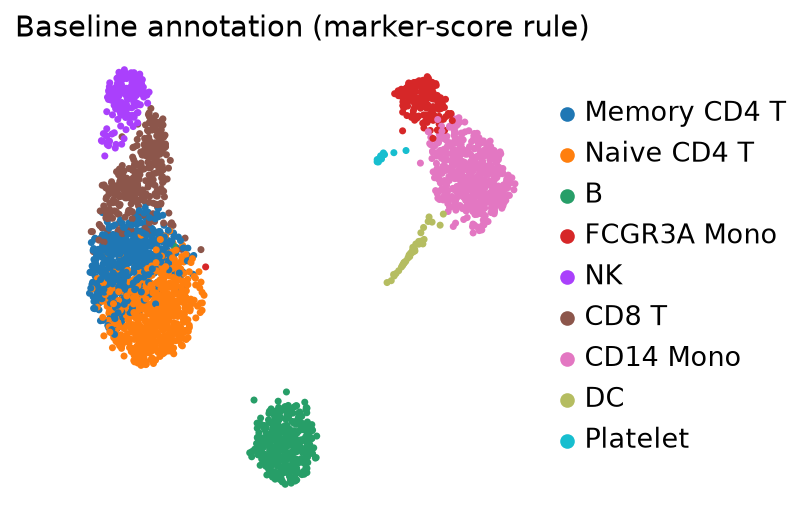
\includegraphics[width=\linewidth]{../single_cell/outputs/umap_s2b_baseline_annotated.png}\\[-2pt]{\small (A)}
\end{minipage}\hfill
\begin{minipage}{0.58\linewidth}\centering
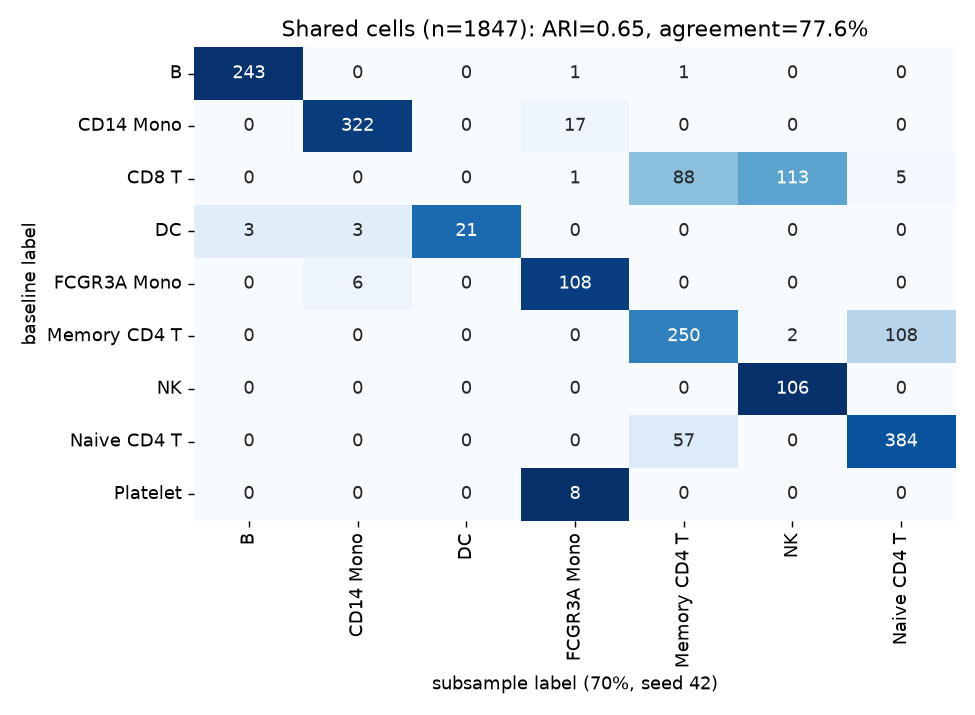
\includegraphics[width=\linewidth]{../single_cell/outputs/fig_s4a_downsample_confusion.png}\\[-2pt]{\small (B)}
\end{minipage}\\[4pt]
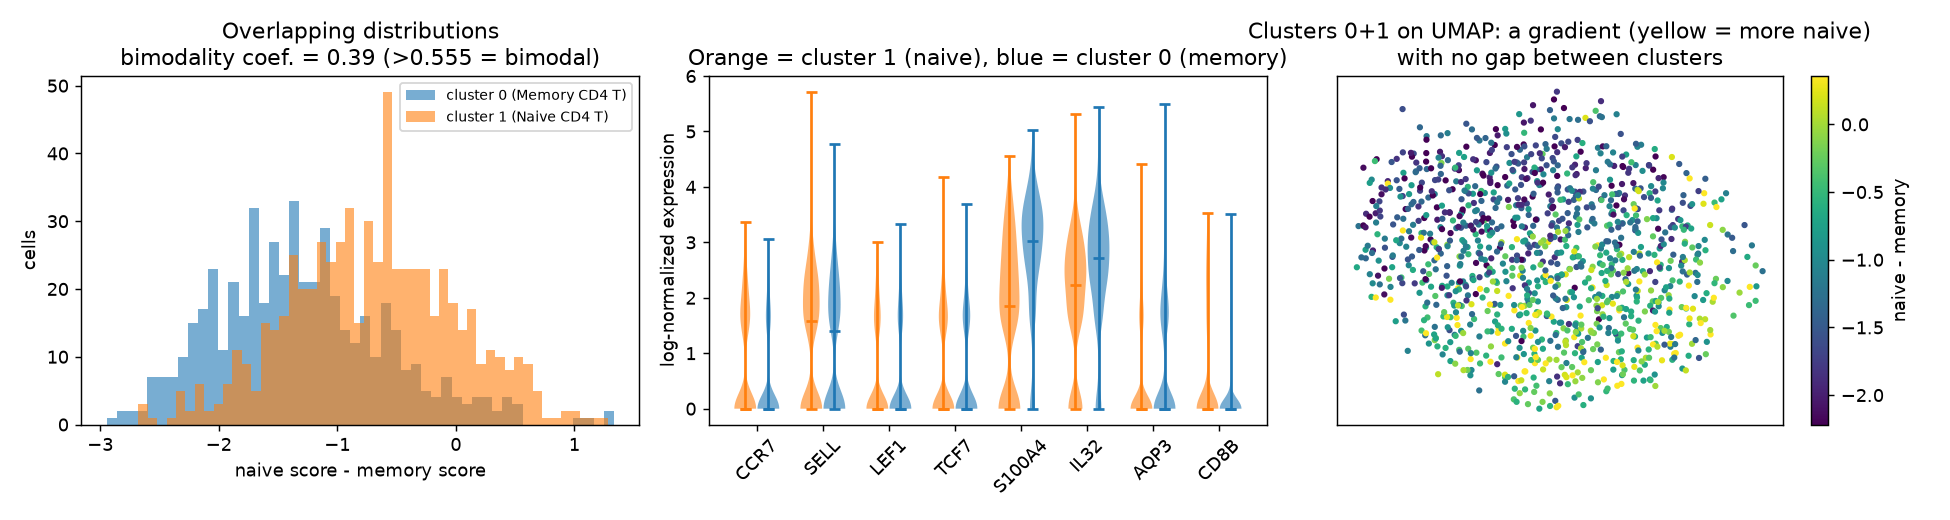
\includegraphics[width=\linewidth]{../single_cell/outputs/fig_s5a_naive_memory_continuum.png}\\[-2pt]{\small (C)}
\caption{\textbf{PBMC3k.} (A) Baseline UMAP with automatic labels. (B) Baseline vs 70\% subsample labels on the 1{,}847 shared cells. (C) Naive-minus-memory score for clusters 0 and 1: overlapping distributions, graded markers and a gradient on the UMAP without a gap.}
\label{fig:sc}
\end{figure}

\paragraph{Resolution and subsampling \obs.} Table~\ref{tab:robust} summarises both checks. Across resolutions, \emph{B cells} are perfectly stable (recall and purity 1.00). NK and CD14 monocyte cells always keep their label, but at low resolution their clusters absorb CD8\,T cells (NK purity 0.36--0.38) or FCGR3A monocytes and DCs. CD8\,T, naive CD4 and memory CD4 exist only at resolution $\ge 1.0$. Changing only the Leiden seed gives ARI 0.77--0.83, mostly from the 2-iteration default (ARI 0.94 when run to convergence); nearly all seed-to-seed change is at the naive/memory boundary. In the 70\% subsample (ARI 0.65, label agreement 77.6\%), CD8\,T cells split between NK (55\%) and memory CD4 (43\%), and the 8 retained platelets joined the FCGR3A monocytes. Re-clustering the same subsample at 1.2, or using five other subsample seeds, recovers CD8\,T every time; platelets return in only 1 of 5.

\begin{table}[t]
\centering\small
\caption{\textbf{Robustness checks} (\code{table\_s3b/c/e/f}, \code{table\_s4a/b/d/e}).}
\label{tab:robust}
\begin{tabular}{@{}l c c c p{6.6cm}@{}}
\toprule
Comparison & Clusters & ARI & NMI & Main change \\
\midrule
Resolution 0.3 vs 1.0 & 5 & 0.59 & 0.77 & T, NK/CD8 and myeloid clusters merge \\
Resolution 0.6 vs 1.0 & 7 & 0.64 & 0.82 & CD8\,T merges with NK; naive+memory CD4 merge \\
Resolution 1.4 vs 1.0 & 11 & 0.70 & 0.80 & naive/memory CD4 re-split (72\% / 82\% kept) \\
Leiden seeds 1--5 & 9 & 0.77--0.83 & -- & naive/memory boundary (0.70--0.93 kept) \\
70\% subsample (seed 42) & 7 & 0.65 & 0.75 & CD8\,T and platelets lost; agreement 77.6\% \\
Subsample seeds 1--5 & 8--9 & -- & -- & CD8\,T 5/5, platelets 1/5; agreement 81--85\% \\
\bottomrule
\end{tabular}
\end{table}

\paragraph{Ambiguous population: naive vs memory CD4 \obs\ \pred.}\label{sec:s5}
Clusters 0 and 1 differ only modestly (cluster 1: ribosomal genes, log$_2$FC 0.25--0.5; cluster 0: S100A4 $-1.7$, S100A11 $-1.5$, IL32 $-1.0$). The naive-minus-memory score is not bimodal (bimodality coefficient 0.39 $<$ 0.555; AUC between clusters 0.73), and 16--21\% of each cluster's kNN edge weight points to the other cluster (Fig.~\ref{fig:sc}C). This matches the continuous naive $\to$ central memory $\to$ effector memory differentiation of CD4 T cells. Cluster 1 also contains CD8 cells: 26\% express CD8A or CD8B, against a background of 3--10\% in B and NK cells and only 60\% detection in true CD8\,T cells, giving an estimated 31--40\% CD8 T cells. Naive CD8 cells share the CCR7/SELL/LEF1 programme and lack cytotoxic genes, so they co-cluster with naive CD4 cells; CD4 mRNA itself is detected in only 9--12\% of CD4 T cells. We therefore relabel cluster 1 ``Naive T, CD4/CD8 mixed''. Protein markers (CITE-seq) would be needed to resolve it.

\subsection{Visium mouse brain: spatial domains}
\paragraph{Domains \obs.} QC kept 2{,}683 of 2{,}702 in-tissue spots (17{,}535 genes). Expression-only clustering gave 16 domains (20--339 spots) that map to contiguous regions (Fig.~\ref{fig:sp}A). Tentative anatomy from marker genes and the Allen atlas~\cite{lein2007} \pred: cortical layers (domains 2, 3, 15), thalamus (4, 5; Tcf7l2, Prkcd), fibre tracts (8; Mbp, Plp1), hippocampus (11--13), hypothalamus (6), ventricle/ependyma (14), meninges (9) and striatum-like (1, probably also containing choroid plexus). Domains 0, 7 and 10 are not annotated with confidence.

\begin{figure}[t]
\centering
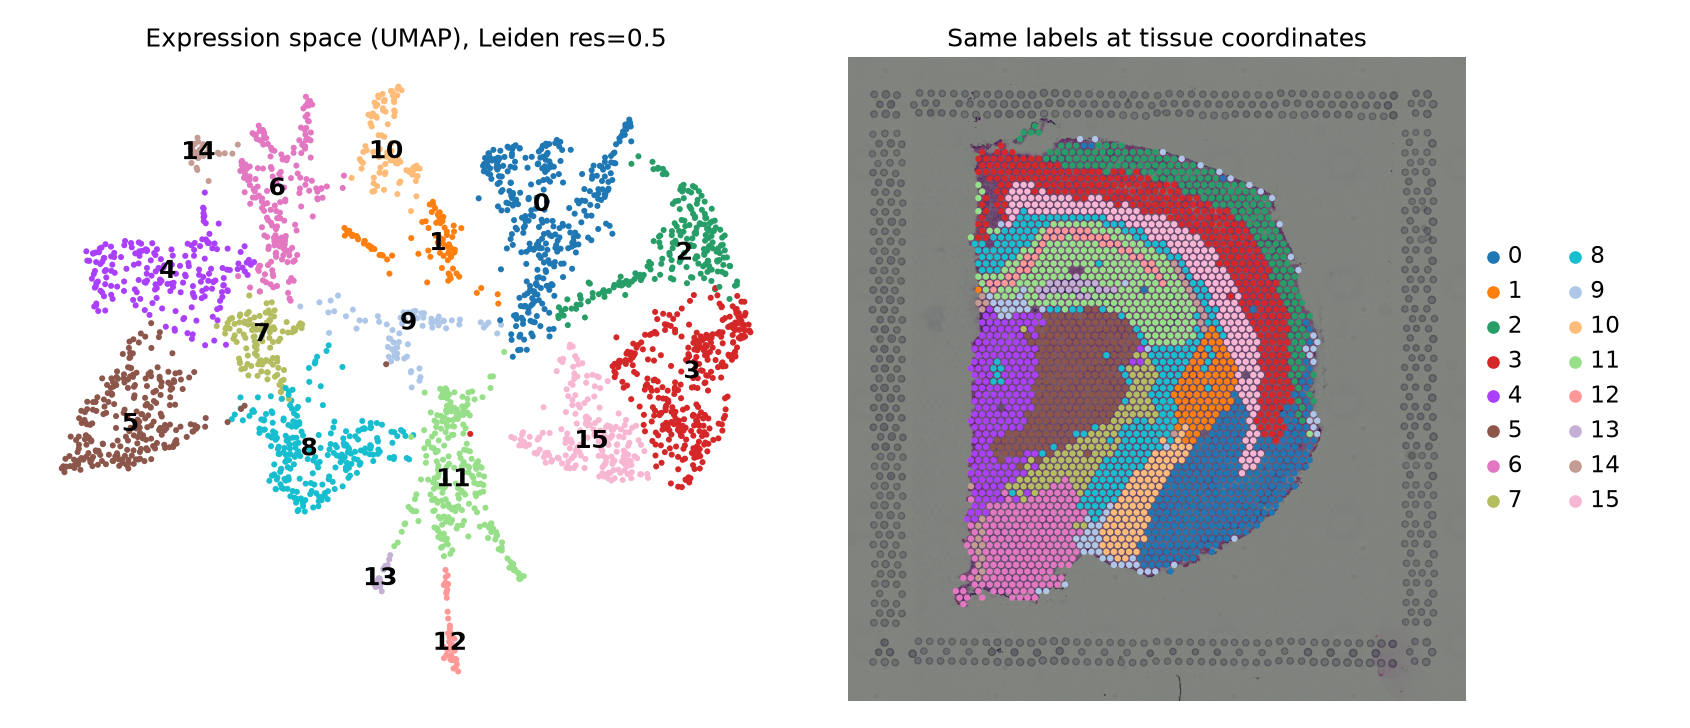
\includegraphics[width=0.92\linewidth]{../spatial/outputs/fig_t1_domains_expression_vs_tissue.png}\\[-2pt]{\small (A)}\\[3pt]
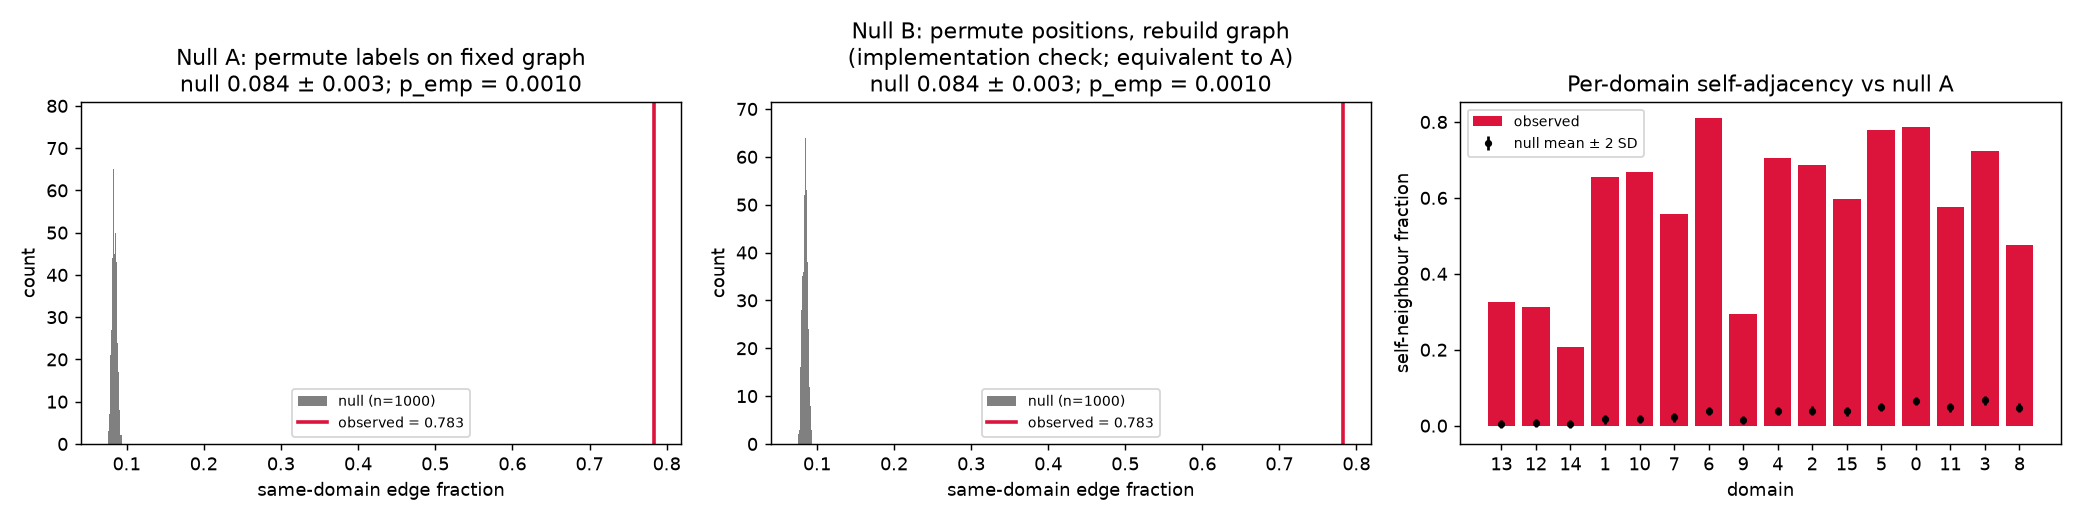
\includegraphics[width=\linewidth]{../spatial/outputs/fig_t5_observed_vs_null.png}\\[-2pt]{\small (B)}
\caption{\textbf{Visium domains.} (A) The same expression-only labels in UMAP space and on tissue. (B) Observed same-domain edge fraction (red) vs 1{,}000 label permutations; the middle panel is the graph-rebuild implementation check, equivalent to the left null; right: per-domain self-adjacency vs null mean $\pm$2\,SD.}
\label{fig:sp}
\end{figure}

\paragraph{Spatial organisation and negative control \obs.} The hexagonal graph has 7{,}759 edges (mean degree 5.78). 78.3\% of edges join spots of the same domain, against 8.4\% under label permutation ($z=224$; no permutation reached the observed value, $p=0.001$, the minimum for $N=1{,}000$; Fig.~\ref{fig:sp}B, Table~\ref{tab:sp}). Every domain is 10--98$\times$ more self-adjacent than expected, and each domain's indicator has Moran's I 0.34--0.88. The strongest between-domain contacts are between hippocampal sub-fields. Sequencing depth and \% mito are themselves spatially structured (Moran's I 0.49 and 0.58) and partly explained by domain ($\eta^2$ 36\% and 31\%). Regressing both out and re-clustering gives 13 domains that agree with the originals (ARI 0.78) and are equally coherent (0.792 vs 0.093).

\begin{table}[t]
\centering\small
\caption{\textbf{Spatial statistics} (\code{table\_t5a}, \code{table\_t5c}, \code{table\_t4b}).}
\label{tab:sp}
\begin{tabular}{@{}l c c c c@{}}
\toprule
Statistic & Observed & Null mean $\pm$ SD & $z$ & Empirical $p$ \\
\midrule
Same-domain edge fraction (16 domains) & 0.783 & 0.084 $\pm$ 0.003 & 224 & 0.001 \\
Same, after depth/mito regression (13 domains) & 0.792 & 0.093 $\pm$ 0.003 & -- & 0.001 \\
\midrule
Spearman $\rho$: Moran's I vs DE (Wilcoxon $z$) & 0.52 & & & $1.5\times10^{-15}$ \\
Spearman $\rho$: Moran's I vs DE (max log$_2$FC) & 0.29 & & & $<10^{-4}$ \\
\bottomrule
\end{tabular}
\end{table}

\paragraph{Spatial genes vs differential expression \obs\ \pred.} All 200 tested HVGs have FDR $<0.05$ for Moran's I, which is expected for pre-selected variable genes, so we use ranks rather than the count. The top spatial genes are Prkcd (I = 0.87, thalamus), Mbp (fibre tracts), Ttr (choroid plexus) and Pmch (Appendix Fig.~\ref{fig:genes}); blood and vascular genes (Ccl5, S100a8/9) rank lowest. Genes high in both rankings mark large regions that match a domain (Prkcd, Mbp). \emph{Agrp} is spatially sharp (Moran rank 7) but ranks 183rd by Wilcoxon $z$: it is confined to the small arcuate region, so most spots of its best domain are zero and the rank-based test penalises it, even though its fold change is large (log$_2$FC 5.5, rank 27). Conversely, Cpne9 separates domains on average (DE rank 30) but varies in a graded way inside them (Moran rank 103). The rankings therefore measure different things, local neighbour agreement vs separation of predefined groups, and their agreement depends on the DE metric.

\section{Discussion and limitations}
Across tasks the most reliable conclusions are the coarse ones: the location of the three EGFR variants relative to the drug and the catalytic machinery, the major PBMC lineages, and the existence of spatially coherent brain domains. Finer conclusions depend on choices that we varied explicitly: the L858R mechanism rests on static structures that carry an engineered V948R, the CD8\,T/NK split and the naive/memory boundary depend on resolution and sampling, and the gene-ranking comparison depends on the DE metric. The main limitations are: (i) no single-mutant T790M--erlotinib complex was analysed and mechanisms are inferred from static structures; (ii) PBMC labels rest on sparse mRNA, so CD4/CD8 identity cannot be resolved without protein data; (iii) the spatial null assumes complete spatial randomness, a weak alternative (a null preserving autocorrelation, such as shifted label maps, was not run), Visium spots mix several cells, and only one section was analysed.

\paragraph{Code and data availability.} Code, outputs and this report: \url{https://github.com/CosmoBean/GenAIBiomedicine}. Run \code{bash submission/run\_all.sh}. Seeds: Task 2 seed 0 (PCA, kNN, Leiden, UMAP), subsample seed 42, extra seeds 1--5; Task 3 seed 0 (clustering, null), seed 1 (graph-rebuild check); Task 1 is deterministic. Data: 10x Genomics PBMC3k and V1\_Adult\_Mouse\_Brain (course repository copies, checksummed); UniProt P00533, P04626, P21860, Q15303; PDB 4HJO, 1M17, 2ITX, 2ITN, 2ITV, 2JIT, 4I22; AlphaFold DB AF-P00533-F1 v6.

\FloatBarrier
\small
\begin{thebibliography}{99}\setlength{\itemsep}{0pt}
\bibitem{cheng2023} Cheng J, et al. Accurate proteome-wide missense variant effect prediction with AlphaMissense. \emph{Science} 381:eadg7492, 2023. PMID 37733863.
\bibitem{gajiwala2013} Gajiwala KS, et al. Insights into the aberrant activity of mutant EGFR kinase domain and drug recognition. \emph{Structure} 21:209--219, 2013. PMID 23273428.
\bibitem{hao2021} Hao Y, et al. Integrated analysis of multimodal single-cell data. \emph{Cell} 184:3573, 2021. PMID 34062119.
\bibitem{jumper2021} Jumper J, et al. Highly accurate protein structure prediction with AlphaFold. \emph{Nature} 596:583--589, 2021. PMID 34265844.
\bibitem{kobayashi2005} Kobayashi S, et al. EGFR mutation and resistance of non-small-cell lung cancer to gefitinib. \emph{N Engl J Med} 352:786--792, 2005. PMID 15728811.
\bibitem{lein2007} Lein ES, et al. Genome-wide atlas of gene expression in the adult mouse brain. \emph{Nature} 445:168--176, 2007. PMID 17151600.
\bibitem{lynch2004} Lynch TJ, et al. Activating mutations in the EGFR underlying responsiveness of NSCLC to gefitinib. \emph{N Engl J Med} 350:2129--2139, 2004. PMID 15118073.
\bibitem{paez2004} Paez JG, et al. EGFR mutations in lung cancer: correlation with clinical response to gefitinib therapy. \emph{Science} 304:1497--1500, 2004. PMID 15118125.
\bibitem{palla2022} Palla G, et al. Squidpy: a scalable framework for spatial omics analysis. \emph{Nat Methods} 19:171--178, 2022. PMID 35102346.
\bibitem{pao2005} Pao W, et al. Acquired resistance of lung adenocarcinomas to gefitinib or erlotinib is associated with a second mutation in the EGFR kinase domain. \emph{PLoS Med} 2:e73, 2005. PMID 15737014.
\bibitem{park2012} Park JH, Liu Y, Lemmon MA, Radhakrishnan R. Erlotinib binds both inactive and active conformations of the EGFR tyrosine kinase domain. \emph{Biochem J} 448:417--423, 2012. PMID 23101586.
\bibitem{shan2012} Shan Y, et al. Oncogenic mutations counteract intrinsic disorder in the EGFR kinase and promote receptor dimerization. \emph{Cell} 149:860--870, 2012. PMID 22579287.
\bibitem{stamos2002} Stamos J, Sliwkowski MX, Eigenbrot C. Structure of the EGFR kinase domain alone and in complex with a 4-anilinoquinazoline inhibitor. \emph{J Biol Chem} 277:46265--46272, 2002. PMID 12196540.
\bibitem{traag2019} Traag VA, Waltman L, van Eck NJ. From Louvain to Leiden: guaranteeing well-connected communities. \emph{Sci Rep} 9:5233, 2019. PMID 30914743.
\bibitem{villani2017} Villani AC, et al. Single-cell RNA-seq reveals new types of human blood dendritic cells, monocytes, and progenitors. \emph{Science} 356:eaah4573, 2017. PMID 28428369.
\bibitem{wolf2018} Wolf FA, Angerer P, Theis FJ. SCANPY: large-scale single-cell gene expression data analysis. \emph{Genome Biol} 19:15, 2018. PMID 29409532.
\bibitem{yun2007} Yun CH, et al. Structures of lung cancer-derived EGFR mutants and inhibitor complexes: mechanism of activation and insights into differential inhibitor sensitivity. \emph{Cancer Cell} 11:217--227, 2007. PMID 17349580.
\bibitem{yun2008} Yun CH, et al. The T790M mutation in EGFR kinase causes drug resistance by increasing the affinity for ATP. \emph{PNAS} 105:2070--2075, 2008. PMID 18227510.
\bibitem{zhang2006} Zhang X, et al. An allosteric mechanism for activation of the kinase domain of epidermal growth factor receptor. \emph{Cell} 125:1137--1149, 2006. PMID 16777603.
\bibitem{zheng2017} Zheng GX, et al. Massively parallel digital transcriptional profiling of single cells. \emph{Nat Commun} 8:14049, 2017. PMID 28091601.
\end{thebibliography}
\normalsize

\clearpage
\appendix
\section{Checkpoint evidence index}\label{app:index}
\begin{table}[H]
\centering\small
\begin{tabularx}{\linewidth}{@{}l l Y@{}}
\toprule
ID & Status & Evidence (page; figure/table; code) \\
\midrule
P1 & complete & p.\,\pageref{sec:map} (Mapping), Table~\ref{tab:p1}; \code{protein/code/01\_map\_and\_measure.py}, \code{table\_p1a--c} \\
P2 & complete & p.\,\pageref{tab:egfr}, Tables~\ref{tab:egfr}, \ref{tab:p2}; \code{01\_map\_and\_measure.py}, \code{02\_mechanism\_checks.py}, \code{table\_p2a--f} \\
P3 & complete & Table~\ref{tab:egfr} and its interpretation (p.\,\pageref{tab:egfr}); references \\
P4 & complete & Fig.~\ref{fig:egfr} (p.\,\pageref{fig:egfr}), Table~\ref{tab:egfr}; \code{03\_render\_structure.py} \\
S1 & complete & Methods; Table~\ref{tab:sc}, Fig.~\ref{fig:sc}A (p.\,\pageref{fig:sc}); Fig.~\ref{fig:qc}; \code{single\_cell/code/01\_qc\_baseline.py} \\
S2 & complete & Table~\ref{tab:sc} (p.\,\pageref{tab:sc}); \code{table\_s2a--d}, \code{dotplot\_\_s2c\_canonical\_markers.png} \\
S3 & complete & Table~\ref{tab:robust} (p.\,\pageref{tab:robust}); \code{02\_resolution\_sweep.py}, \code{table\_s3a--f}, \code{fig\_s3a} \\
S4 & complete & Table~\ref{tab:robust}, Fig.~\ref{fig:sc}B; \code{03\_downsample.py}, \code{table\_s4a--e} \\
S5 & complete & \S\ref{sec:s5}, Fig.~\ref{fig:sc}C, Table~\ref{tab:s5}; \code{04\_ambiguous\_population.py}, \code{table\_s5a--d} \\
T1 & complete & Fig.~\ref{fig:sp}A (p.\,\pageref{fig:sp}); \code{spatial/code/01\_expression\_domains.py}, \code{table\_t1*} \\
T2 & complete & Fig.~\ref{fig:sp}B, Table~\ref{tab:sp} (p.\,\pageref{tab:sp}); \code{02\_spatial\_statistics\_and\_null.py}, \code{table\_t2a--d} \\
T3 & complete & Fig.~\ref{fig:genes}; \code{03\_svg\_vs\_de.py}, \code{table\_t3a--b} \\
T4 & complete & Table~\ref{tab:sp}, Table~\ref{tab:t4}, Fig.~\ref{fig:genes}; \code{table\_t3b\_t4\_moran\_and\_DE\_rankings.csv}, \code{table\_t4b} \\
T5 & complete & Fig.~\ref{fig:sp}B, Table~\ref{tab:sp}; \code{02\_spatial\_statistics\_and\_null.py}, \code{04\_depth\_confound\_check.py}, \code{table\_t5a--d} \\
A & complete$^*$ & Appendix~\ref{app:audit} ($^*$student verification boxes to be completed by the student) \\
R & complete & \code{README.md}, \code{run\_all.sh}, \code{fetch\_data.sh}, \code{requirements.txt}; seeds in \S4 \\
\bottomrule
\end{tabularx}
\end{table}

\section{Agent audits}\label{app:audit}
Agent workspace: Claude Code (Anthropic) with model Claude Opus 5.5, with shell, Python and web access. After the analysis, three independent reviewer agents (one per task) re-derived the key numbers from scratch; issues they found are listed as weaknesses below.

\subsection{Task 1 (EGFR)}
\textbf{Sources.} UniProt P00533 (v301) and paralogs P04626, P21860, Q15303; RCSB PDB 4HJO, 1M17, 2ITX, 2ITN, 2ITV, 2JIT, 4I22; AlphaFold DB AF-P00533-F1 v6 (model, pLDDT, AlphaMissense); 13 papers, each verified on PubMed.\\
\textbf{Computed vs retrieved.} \emph{Computed:} sequence checks, SEQRES-to-UniProt mapping, all distances, neighbour shells, SASA, B-factors, backbone angles, $\alpha$C state, superpositions, paralog alignment. \emph{Retrieved:} sequences and annotations, coordinates, SEQADV records, pLDDT, AlphaMissense scores, and the published mechanisms.\\
\textbf{Independent checks.} (1) Mapping vs the depositors' SEQADV records: 4HJO lists Arg924 as engineered V948, confirming the $-24$ offset, and 2ITN/2ITV/2JIT list S719/R858/M790 at canonical numbers; all agree. (2) All 13 citations resolved to the expected title and journal on PubMed. One newly added PMID was wrong and was corrected by this check.\\
\textbf{Weaknesses found.} \emph{Mapping bug:} aligning only resolved residues gave an inconsistent offset for 2ITX/2ITV; fixed by aligning full SEQRES. \emph{Misleading first result:} apo Met790 superposition suggested a steric clash; tested against drug-bound 4I22, which shows none. \emph{Selective description (review):} L858's charged neighbours and the 4I22 counter-evidence were initially omitted; both are now reported and confidence lowered. \emph{Cut-offs:} M766 at 4.57\,\AA\ sits near the 4.5/5\,\AA\ contact thresholds.
\studentbox{open 4HJO at RCSB, confirm Leu834 is canonical L858, measure Thr766--erlotinib in Mol* and compare with 3.48\,\AA. Result: \underline{\hspace{6cm}}}

\subsection{Task 2 (PBMC3k)}
\textbf{Sources.} PBMC3k filtered matrix (10x Genomics via course repository, SHA-256 checked); marker biology from~\cite{zheng2017,hao2021,villani2017}; methods~\cite{wolf2018,traag2019}. No reference labels or cell-type databases.\\
\textbf{Computed vs retrieved.} \emph{Computed:} QC, normalisation, HVGs, PCA, kNN, UMAP, Leiden, Wilcoxon markers, marker-set scores, ARI/NMI, contingency tables, subsampling, seed sweeps, bimodality coefficient, kNN mixing, CD8 detection rates. \emph{Retrieved:} canonical marker lists and the biology linking markers to cell types.\\
\textbf{Independent checks.} (1) Seed-only control: ARI 0.77--0.83 between seeds (0.94 when Leiden runs to convergence), which calibrates the resolution and subsample effects. (2) The CD8 loss after subsampling was re-tested at resolution 1.2 and with five subsample seeds: CD8\,T was recovered every time, so it is a threshold effect, not a missing population.\\
\textbf{Weaknesses found.} \emph{Mislabelled cluster:} the rule called cluster 1 ``Naive CD4 T''; 26\% of its cells express CD8 (31--40\% after detection correction), so it was relabelled. The first fix (``CD4-dominant'') ignored CD8 dropout and was corrected after review. \emph{Post-hoc resolution:} 1.0 was chosen after seeing 0.6. \emph{Overclaimed stability (review):} recall-only stability hid NK clusters that are 62--64\% CD8\,T at low resolution; purity was added. \emph{Figure errors:} Fig.~\ref{fig:sc}C first had colours reversed between panels and a saturated colour scale; both fixed.
\studentbox{from \code{table\_s2b\_top10\_markers.csv} alone, assign clusters 2, 4 and 6; then rerun \code{03\_downsample.py} and confirm the 77.6\% agreement. Result: \underline{\hspace{6cm}}}

\subsection{Task 3 (Visium)}
\textbf{Sources.} 10x Genomics V1 Adult Mouse Brain matrix and spatial archive (course repository, SHA-256 checked); squidpy~\cite{palla2022}; Allen Mouse Brain Atlas~\cite{lein2007}.\\
\textbf{Computed vs retrieved.} \emph{Computed:} QC, HVGs, PCA, kNN, Leiden domains, UMAP, hexagonal graph, same-domain edge fraction, neighbourhood enrichment, Moran's I, Wilcoxon DE, rank correlations, permutation null, depth/mito regression. \emph{Retrieved:} anatomical meaning of marker genes.\\
\textbf{Independent checks.} (1) The permutation mean (0.0844) matches the analytic expectation $\sum_k n_k(n_k-1)/(N(N-1)) = 0.0844$, confirming the null code. (2) A reviewer rebuilt the hexagonal graph by hand from array coordinates and obtained the same 7{,}759 edges and statistic 0.7832. (3) The absence of coordinates during clustering is enforced by assertions.\\
\textbf{Weaknesses found.} \emph{Null B bug (review):} the coordinate-shuffle null rebuilt its graph from array coordinates, on which the grid mode keeps only 4 neighbours (5{,}178 edges), so it was compared on a different graph (z 182 instead of 224). It now uses the same coordinates, asserts an identical edge count, and is reported as an implementation check because it is equivalent to label permutation. \emph{DE-metric dependence (review):} only the Wilcoxon-$z$ ranking was reported; the fold-change ranking lowers $\rho$ from 0.52 to 0.29 and is now shown. \emph{Weak null:} complete spatial randomness only. \emph{Anatomy:} inferred from markers, not checked against atlas images.
\studentbox{compare two domains in Fig.~\ref{fig:sp}A with the Allen Brain Atlas coronal reference and their markers in \code{table\_t1c}; record whether the labels hold. Result: \underline{\hspace{6cm}}}

\section{Supplementary tables and figures}

\begin{table}[H]
\centering\small
\caption{\textbf{Structure mapping} (\code{table\_p1b}). Offset = author $-$ canonical numbering.}
\label{tab:p1}
\begin{tabular}{@{}l l c l l@{}}
\toprule
PDB & Content & Offset & G719 / T790 / L858 residue & Mismatches vs UniProt \\
\midrule
4HJO & WT(+V948R), erlotinib, inactive & $-24$ & Gly695 / Thr766 / Leu834 & R948 (engineered) \\
1M17 & WT, erlotinib, active-like & $-24$ & Gly695 / Thr766 / Leu834 & none \\
2ITX & WT, AMP-PNP & 0 & Gly / Thr / Leu & none \\
2ITN & G719S, AMP-PNP & 0 & \textbf{Ser} / Thr / Leu & S719 \\
2ITV & L858R, AMP-PNP & 0 & Gly / Thr / \textbf{Arg} & R858 \\
2JIT & T790M, apo & 0 & Gly / \textbf{Met} / Leu & M790 \\
4I22 & L858R/T790M/V948R, gefitinib & 0 & Gly / \textbf{Met} / \textbf{Arg} & M790, R858, R948 \\
AF v6 & AlphaFold model; pLDDT & 0 & 73.3 / 88.4 / 51.2 & none \\
\bottomrule
\end{tabular}
\end{table}

\begin{table}[H]
\centering\small
\caption{\textbf{Site measurements in three reference structures} (\AA; full table for 8 structures in \code{table\_p2a}).}
\label{tab:p2}
\begin{tabular}{@{}l l c c c c c c@{}}
\toprule
Structure & Site & $\to$ ligand & $\to$ K745 NZ & $\to$ E762 & $\to$ D855 & $\to$ $\alpha$C & rel.\ SASA \\
\midrule
4HJO (K--E 13.3) & G719 & 5.06 & 7.78 & 20.35 & 10.02 & 16.5 & 0.35 \\
 & T790 & 3.48 & 9.03 & 14.27 & 8.57 & 7.5 & 0.21 \\
 & L858 & 5.26 & 3.58 & 6.18 & 2.96 & 4.57 & 0.10 \\
1M17 (K--E 3.05) & G719 & 4.50 & 9.57 & 12.41 & 10.89 & 12.3 & 0.37 \\
 & T790 & 3.41 & 8.56 & 7.38 & 9.03 & 3.2 & 0.17 \\
 & L858 & 10.12 & 8.70 & 6.64 & 5.04 & 6.6 & 0.15 \\
2ITX (K--E 3.58) & G719 & 4.27 & 10.17 & 13.10 & 11.93 & 13.0 & 0.35 \\
 & T790 & 3.13 & 7.10 & 6.62 & 9.85 & 3.9 & 0.15 \\
 & L858 & 6.27 & 10.17 & 6.81 & 4.94 & 6.2 & 0.25 \\
\bottomrule
\end{tabular}
\end{table}

\begin{table}[H]
\centering\small
\caption{\textbf{Marker detection (\% of cells) in T-cell clusters} (\code{table\_s5b}, \code{table\_s5d}).}
\label{tab:s5}
\begin{tabular}{@{}l c c c@{}}
\toprule
Genes & Cluster 0 ``memory'' & Cluster 1 ``naive'' & Cluster 5 CD8 T \\
\midrule
CCR7 / SELL / LEF1 & 27 / 51 / 28 & 44 / 60 / 35 & 6 / 31 / 7 \\
S100A4 / IL32 / AQP3 & 91 / 91 / 38 & 69 / 78 / 26 & 96 / 96 / 19 \\
CD4 & 12 & 9 & 4 \\
CD8A or CD8B & 11 & 26 & 60 \\
GZMK / CCL5 & 9 / 28 & 5 / 18 & 57 / 97 \\
\bottomrule
\end{tabular}
\end{table}

\begin{table}[H]
\centering\small
\caption{\textbf{Spatial vs DE ranking examples} (rank among 200 genes; \code{table\_t3b\_t4\_moran\_and\_DE\_rankings.csv}).}
\label{tab:t4}
\begin{tabular}{@{}l l c c c c@{}}
\toprule
Category & Gene & Moran rank & DE rank ($z$) & DE rank (log$_2$FC) & \% spots detected \\
\midrule
High in both & Prkcd & 1 & 1 & 41 & 53 \\
 & Mbp & 2 & 2 & 102 & 100 \\
Spatial-high, DE($z$)-low & Agrp & 7 & 183 & 27 & 4 \\
 & Gm5741 & 10 & 190 & 97 & 4 \\
 & Fezf1 & 22 & 161 & 62 & 5 \\
DE-high, spatial-lower & Cpne9 & 103 & 30 & 171 & 42 \\
\bottomrule
\end{tabular}
\end{table}

\begin{figure}[H]
\centering
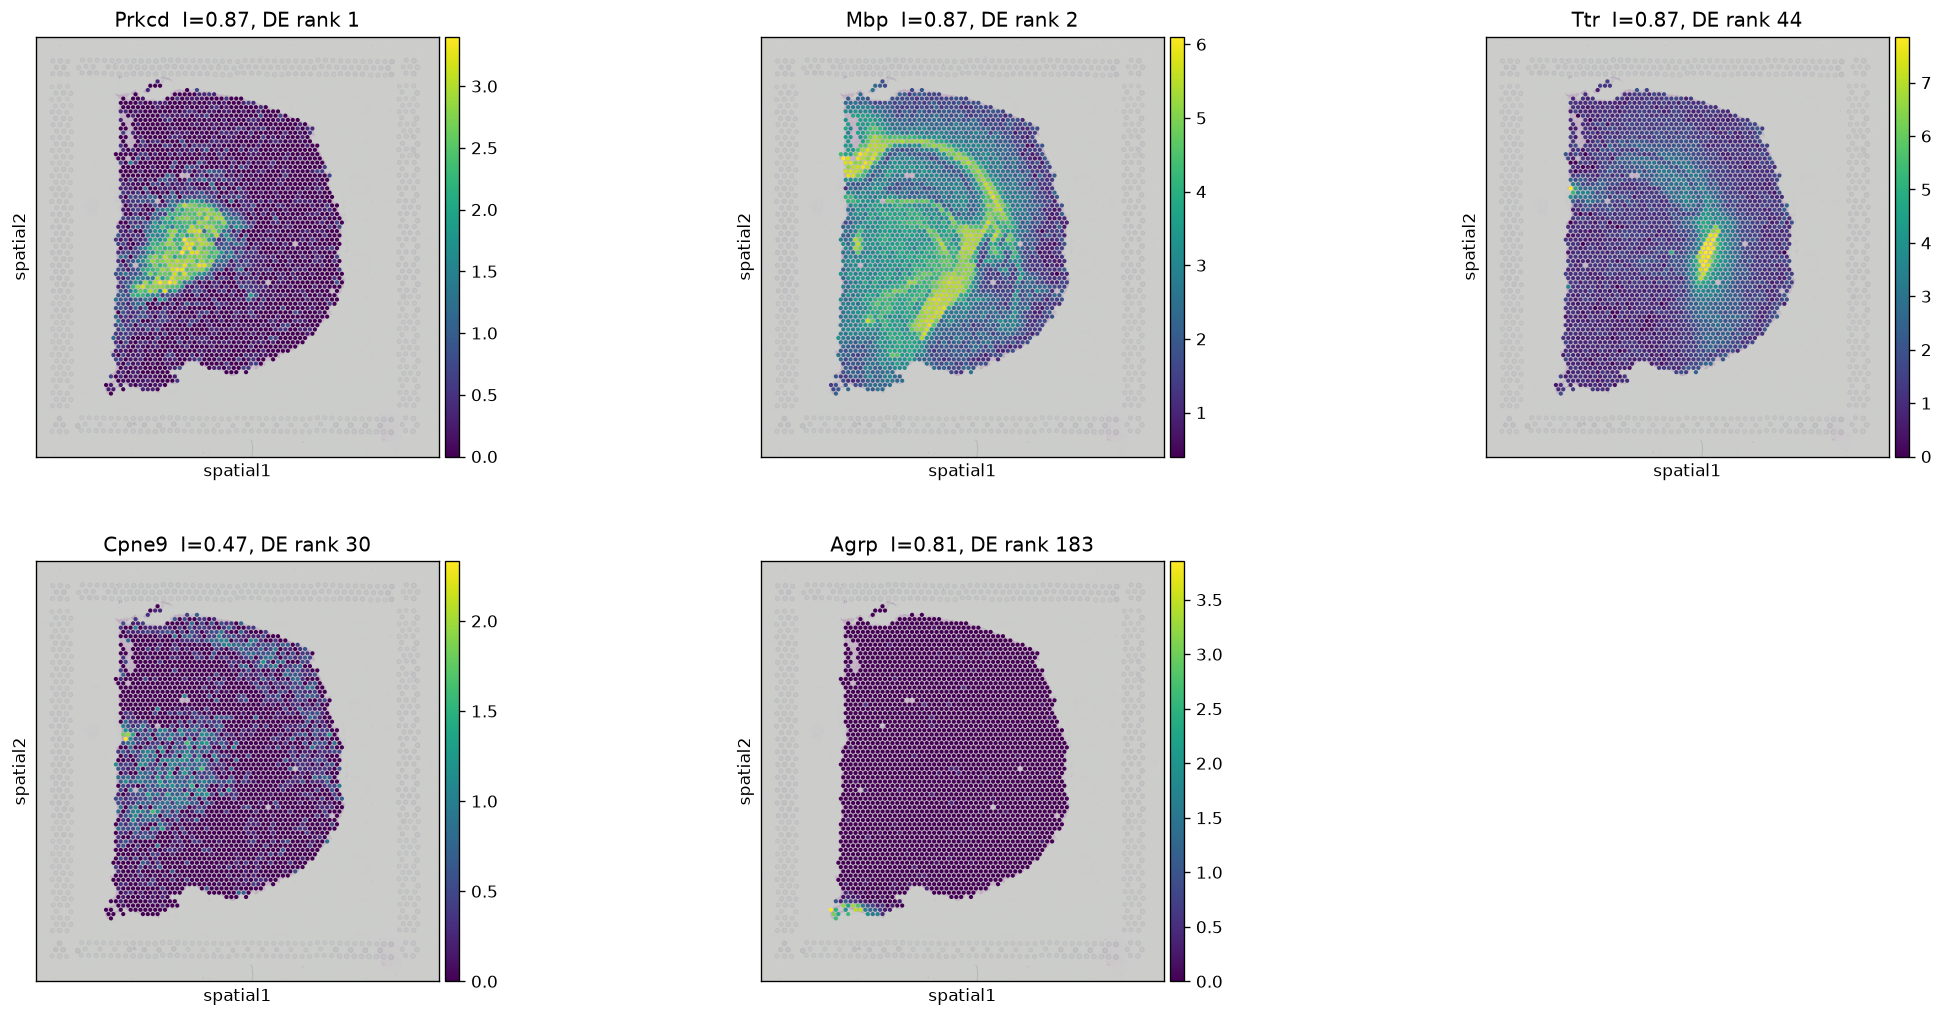
\includegraphics[width=0.9\linewidth]{../spatial/outputs/fig_t3_selected_genes_on_tissue.png}
\caption{\textbf{Selected genes on tissue}, with Moran's I and Wilcoxon-$z$ DE rank.}
\label{fig:genes}
\end{figure}

\begin{figure}[H]
\centering
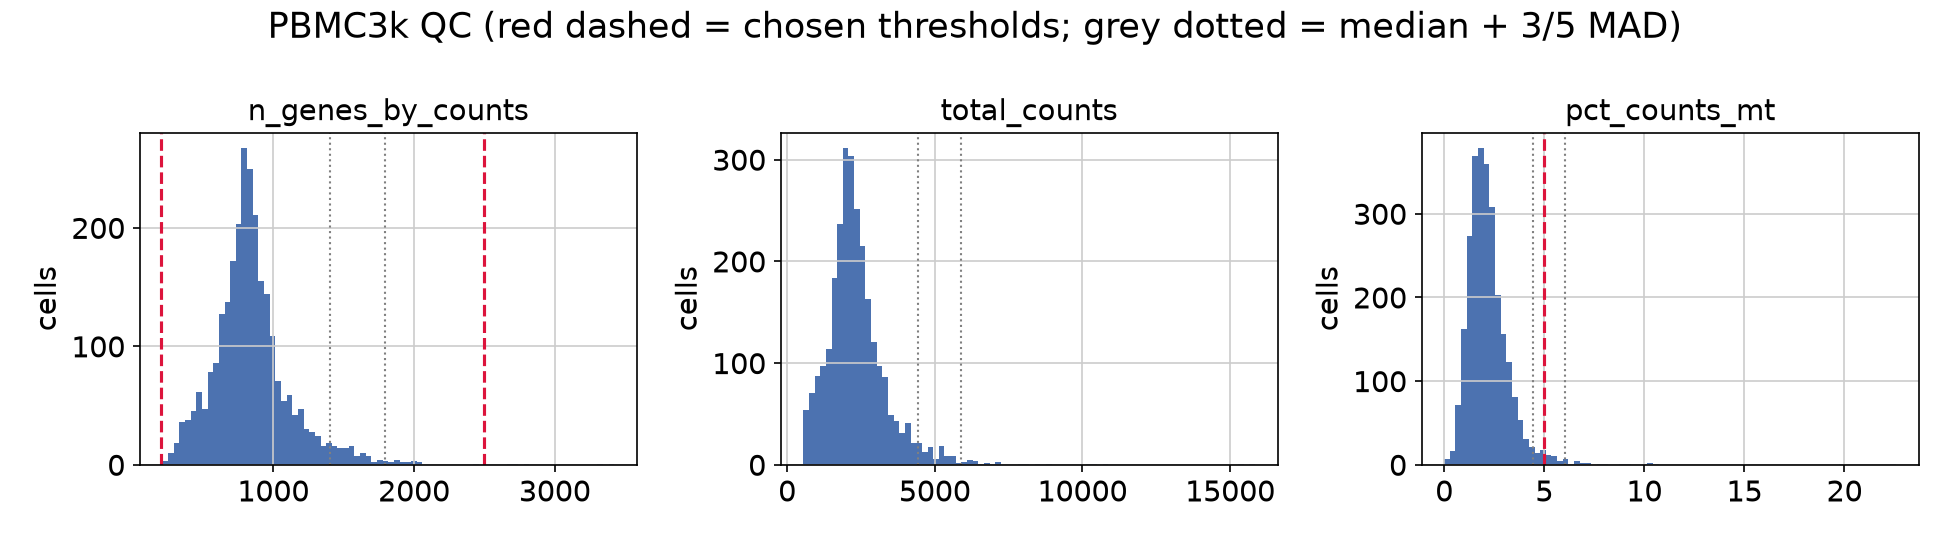
\includegraphics[width=0.85\linewidth]{../single_cell/outputs/fig_s1a_qc_histograms.png}
\caption{\textbf{PBMC3k QC distributions} with thresholds (red) and median + 3/5 MAD (grey). Medians: 817 genes, 2{,}197 UMIs, 2.03\% mito; the cuts remove 5 cells ($>$2{,}500 genes) and 57 cells ($\ge$5\% mito).}
\label{fig:qc}
\end{figure}

\end{document}
